\capitulo{5}{Resultados}

\section{Resumen de resultados}

El desarrollo del sistema de monitoreo cardíaco en tiempo real junto al modelo de predicción ha permitido la creación de una herramienta efectiva para la supervisión continua de la actividad cardíaca. Los objetivos establecidos al inicio del proyecto se han cumplido de la siguiente manera:

1. \textbf{Conexión estable vía USB}: La comunicación entre el Arduino y la aplicación web se realiza mediante una conexión USB, la cual quizás no es la más óptima en cuanto a comodidad y manejabilidad, pero viendo el lado positivo se elimina la necesidad de baterías y se garantiza una transmisión de datos constante y fiable.

2. \textbf{Monitoreo continuo de la actividad cardíaca}: El sistema desarrollado permite la visualización en tiempo real de los datos de ECG, proporcionando una herramienta útil para la detección temprana de irregularidades cardíacas.

3. \textbf{Accesibilidad y facilidad de uso}: La interfaz web creada con Streamlit es intuitiva y accesible, permitiendo a los usuarios sin conocimientos técnicos manejar el sistema con facilidad (Figura \ref{fig:interfaz}).

4. \textbf{Predicción del tipo de ciclo cardíaco}: Utilizando modelos de machine learning, el sistema puede realizar predicciones que clasifican cada ciclo cardíaco (latido de paciente), pudiendo así detectar alguna anomalía, aunque la precisión está limitada por la calidad de los datos de entrenamiento disponibles (Figura \ref{fig:analisis}).

Aun asi la parte positiva es que conocer los tipos de latidos del paciente nos da información valiosa para la evaluación y gestión de la salud cardíaca. A continuación, se detallan algunos beneficios específicos:

Identificar patrones anormales en los latidos, como latidos de ectopia supraventricular o ventricular, puede ayudar en el diagnóstico temprano de arritmias y otras condiciones cardíacas.
Detectar y clasificar latidos anormales puede prevenir complicaciones graves como infartos de miocardio, fibrilación auricular y otras arritmias potencialmente peligrosas.

5. \textbf{Almacenamiento y análisis de datos}: Se ha implementado una base de datos SQLite para almacenar las predicciones, facilitando que se pueda descargar en un archivo \textbf{.csv} para la generación de estadísticas (Figura \ref{fig:bbdd}).


\begin{figure}[h]
\centering
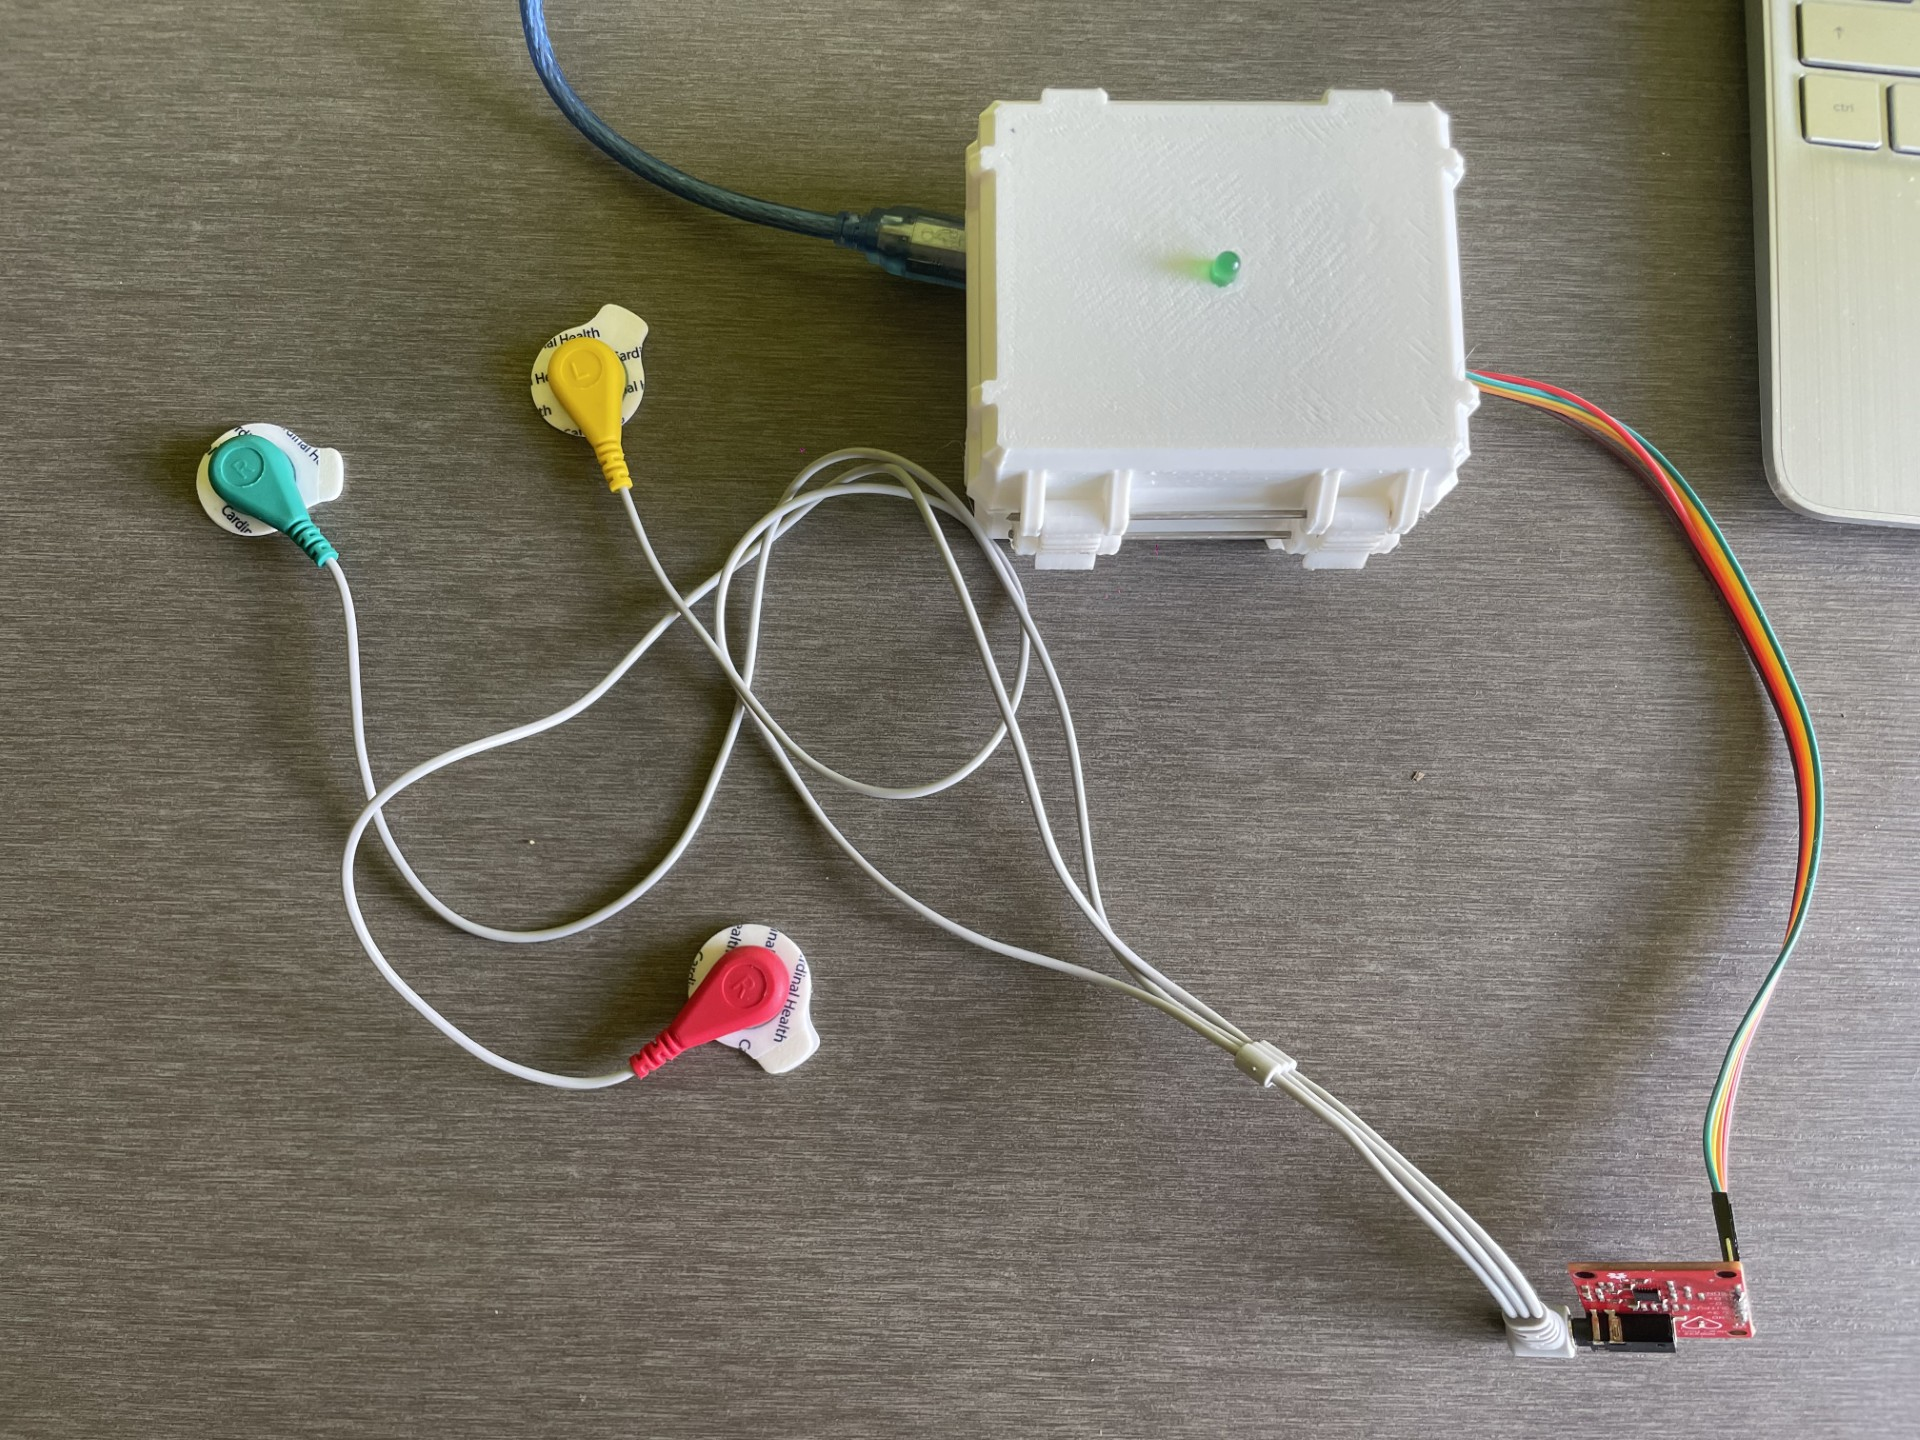
\includegraphics[width=0.8\textwidth]{img/proyecto.jpg}
\caption{Hardware del sistema de monitoreo cardíaco, mostrando el Arduino conectado al sensor de ECG (Fuente propia).}
\label{fig:hardware}
\end{figure}

\begin{figure}[h]
\centering
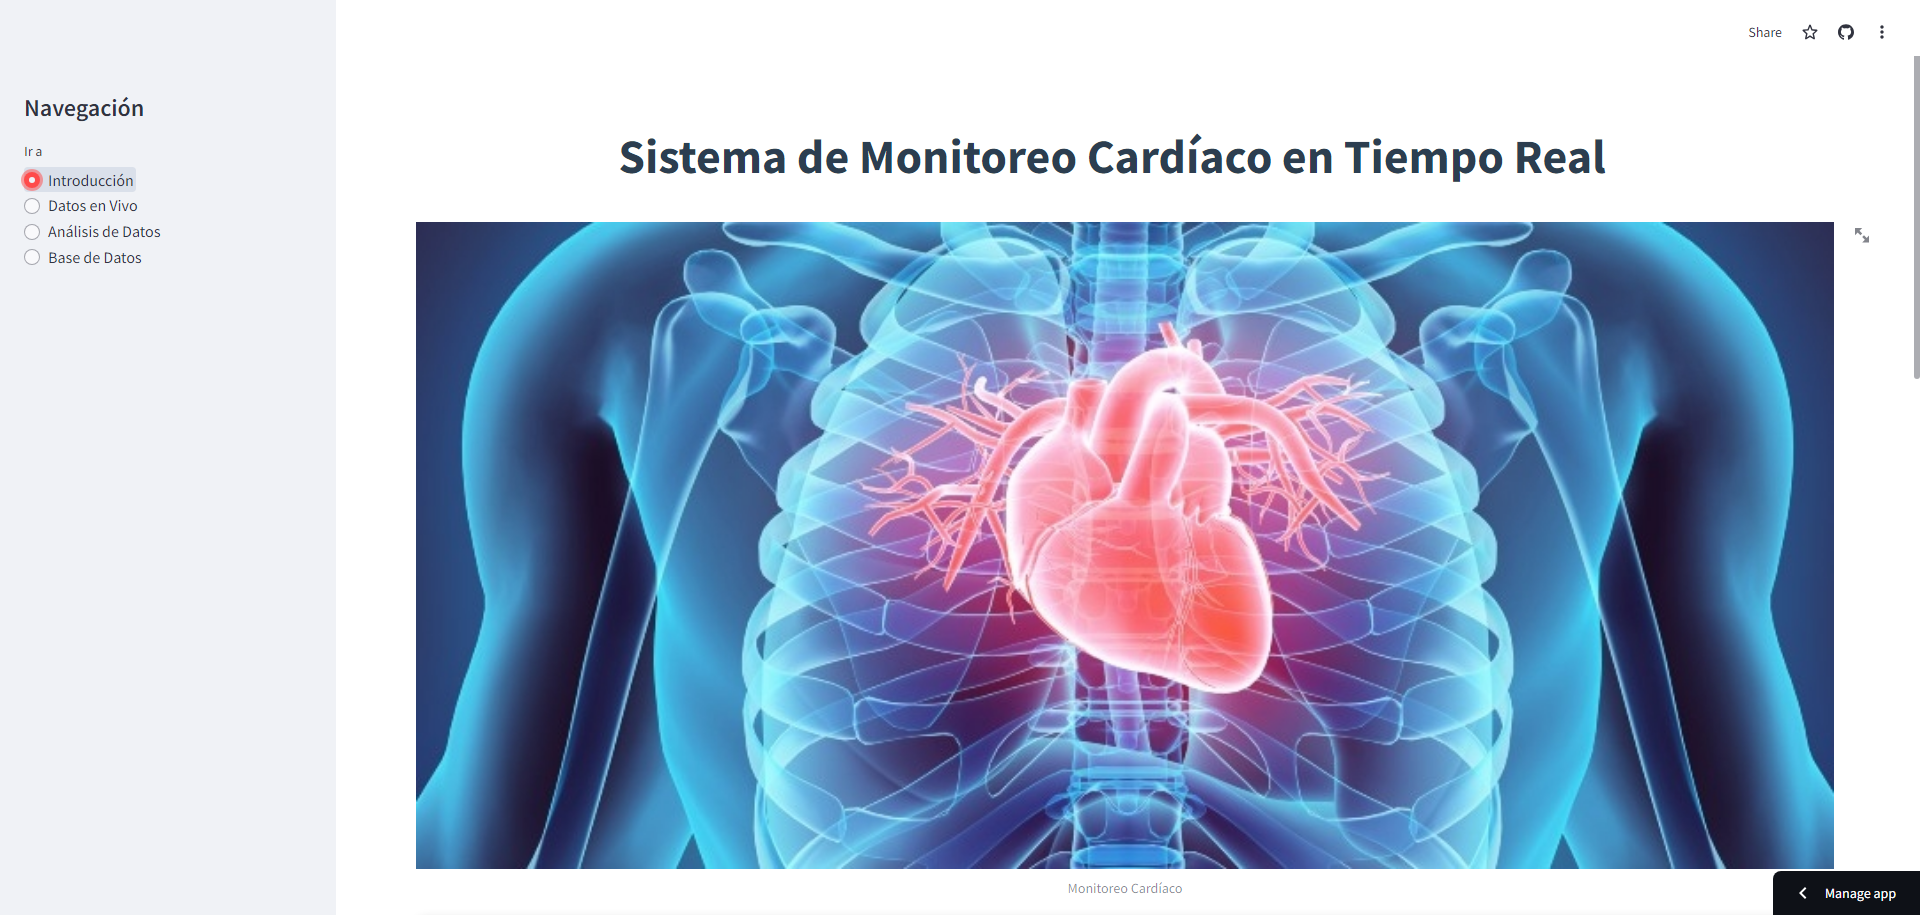
\includegraphics[width=0.8\textwidth]{img/interfaz_streamlit.png}
\caption{Interfaz de la aplicación web creada en Streamlit (Fuente propia).}
\label{fig:interfaz}
\end{figure}

\begin{figure}[h]
\centering
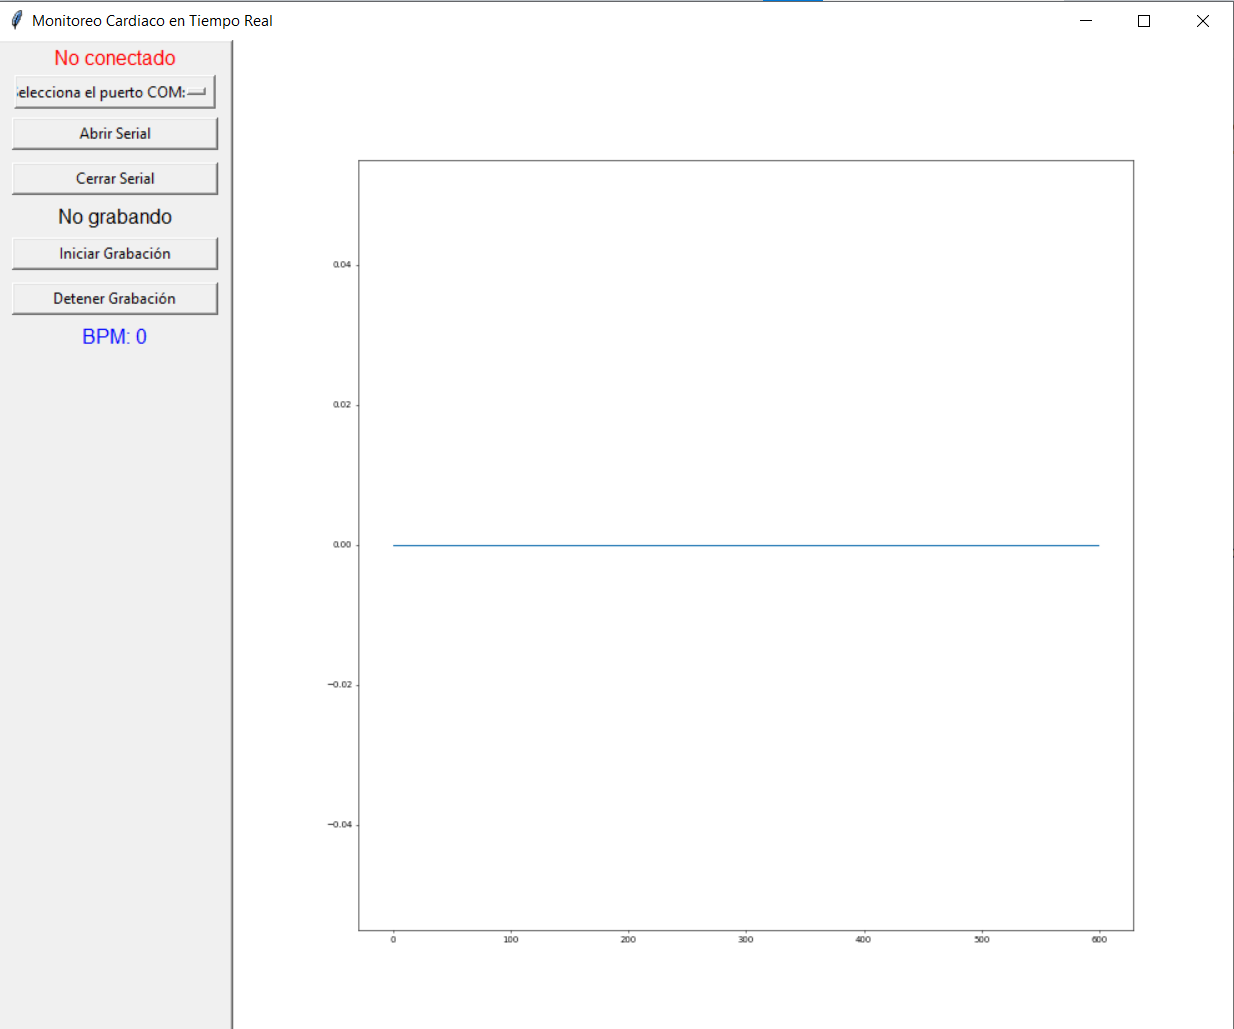
\includegraphics[width=0.8\textwidth]{img/ventana_tinker.png}
\caption{Ventana de visualización y grabación de datos en vivo en la aplicación web (Fuente propia).}
\label{fig:ventana}
\end{figure}

\begin{figure}[h]
\centering
\begin{minipage}[b]{0.45\textwidth}
\centering
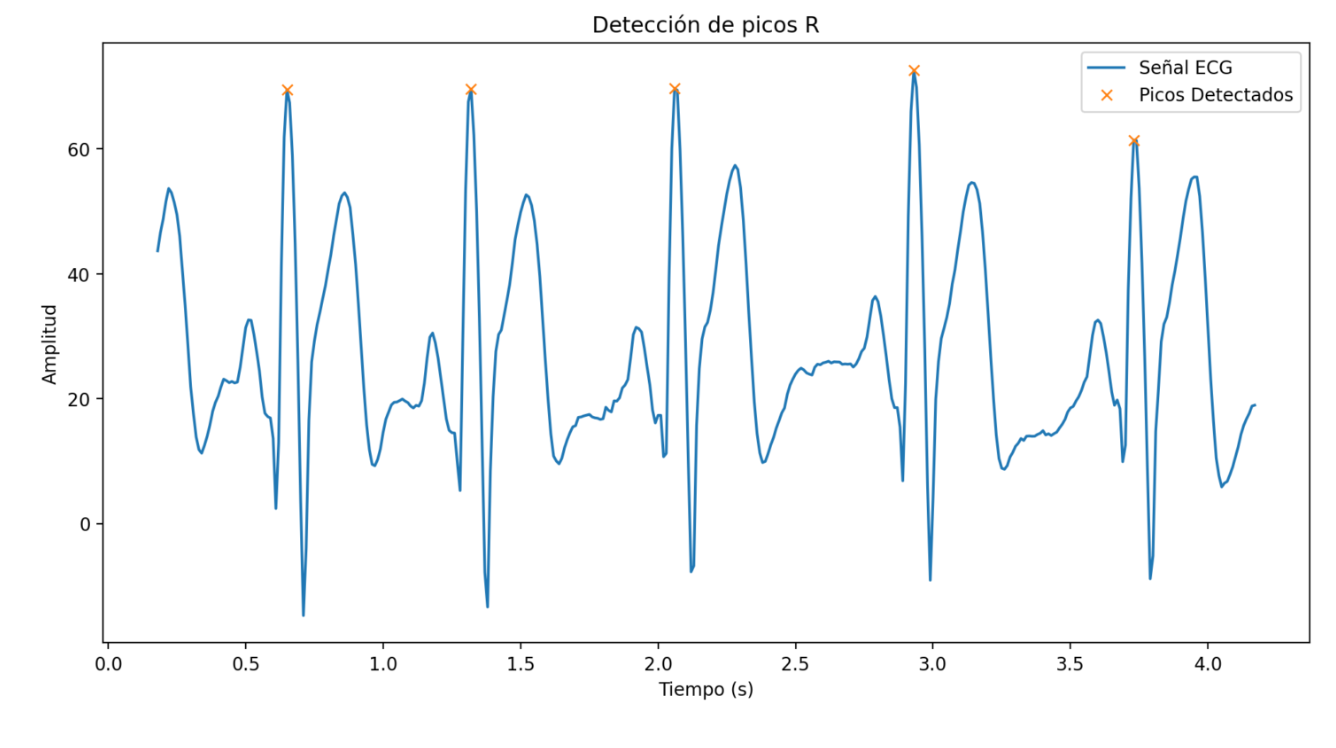
\includegraphics[width=\textwidth]{img/analisis1.png}
\caption{Apartado donde se detectan los picos R de cada ciclo cardíaco para segmentar y realizar la predicción de datos de ECG introducidos en la aplicación web (Fuente propia).}
\label{fig:analisis1}
\end{minipage}
\hfill
\begin{minipage}[b]{0.45\textwidth}
\centering
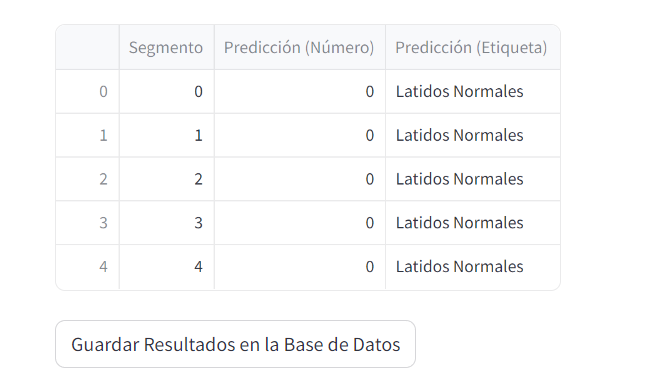
\includegraphics[width=\textwidth]{img/analisis2.png}
\caption{Tabla con los resultados de la predicción que clasifica cada tipo de ciclo cardíaco de la muestra introducida en la aplicación web (Fuente propia).}
\label{fig:analisis2}
\end{minipage}
\caption{Ventana de análisis de datos de ECG en la aplicación web.}
\label{fig:analisis}
\end{figure}

\begin{figure}[h]
\centering
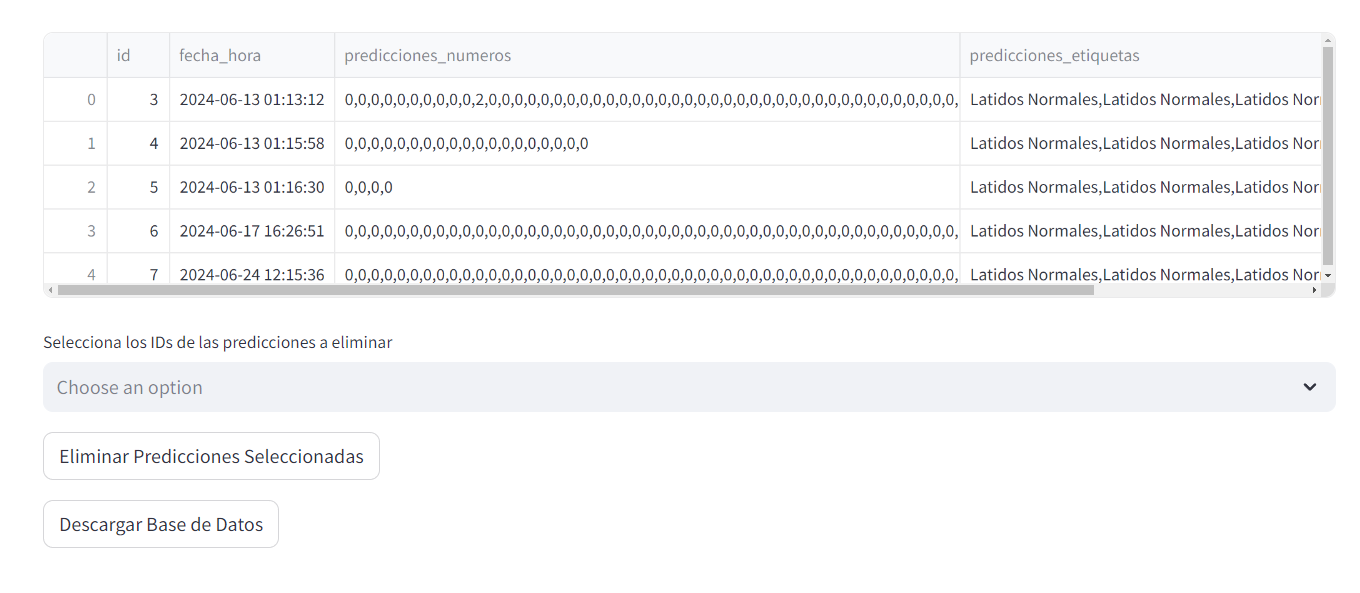
\includegraphics[width=0.8\textwidth]{img/bbdd.png}
\caption{Ventana de almacenamiento de las predicciones en la base de datos de la aplicación web (Fuente propia).}
\label{fig:bbdd}
\end{figure}

El prototipo puede llegar a ser una herramienta prometedora para el monitoreo cardíaco, pero hay áreas que requieren mejoras adicionales, especialmente en la precisión de las predicciones y la calidad de los datos que utiliza el modelo como entrenamiento.

\section{Discusión}

Los resultados de este proyecto representan un avance significativo en el campo del monitoreo cardíaco en tiempo real. A continuación, se discuten los aspectos más destacados y las áreas de mejora, basados en la implementación y los resultados obtenidos.

Uno de los logros más importantes es la creación de una interfaz web intuitiva y accesible mediante Streamlit, que permite a los usuarios sin conocimientos técnicos supervisar la actividad cardíaca en tiempo real (Figura \ref{fig:ventana}). La facilidad de uso y la capacidad de visualización en tiempo real proporcionan una herramienta valiosa tanto para profesionales de la salud como para pacientes.

La implementación de un sistema de predicción basado en machine learning es otro avance clave. Utilizando modelos de Random Forest, el sistema puede clasificar cada ciclo cardíaco y detectar anomalías, lo cual es esencial para la prevención y diagnóstico temprano de enfermedades cardíacas. Como se detalla en la sección de resultados, conocer y clasificar los tipos de latidos cardíacos es crucial para un manejo integral de la salud cardíaca (Figura \ref{fig:analisis}). Esto permite diagnósticos más precisos, tratamientos personalizados y una mejor prevención de enfermedades cardíacas graves.

Sin embargo, se identificaron varias áreas que requieren mejoras adicionales. La precisión del modelo de predicción está limitada por la calidad y cantidad de los datos de entrenamiento disponibles. Es fundamental mejorar la calidad de los datos y aumentar el conjunto de datos de entrenamiento para mejorar la robustez y precisión del modelo.

Además, aunque la conexión USB utilizada garantiza una transmisión de datos fiable, no es la opción más cómoda para el usuario. Implementar una conexión inalámbrica estable, como Bluetooth o WiFi, sería un paso importante para mejorar la comodidad y movilidad del sistema.

Para evaluar la facilidad de uso de la aplicación web creada, se utilizó la Escala de Usabilidad del Sistema (SUS). La SUS es una herramienta sencilla que, mediante un cuestionario de diez preguntas, permite evaluar rápidamente distintos aspectos de la usabilidad de la web. Este cuestionario examina puntos como la facilidad de uso, la eficiencia y la satisfacción del usuario, lo que hace que los resultados y las conclusiones obtenidas sean más válidos y confiables \cite{Brooke}. Realizar esta evaluación proporciona una visión de la efectividad y usabilidad del proyecto en general y ayuda mucho a identificar posibles áreas de mejora. La encuesta y sus resultados pueden consultarse en el Anexo G-Estudio experimental

En conclusión, en este proyecto se ha desarrollado un sistema de monitoreo cardíaco en tiempo real que ofrece herramientas para el análisis de los datos. Aunque se han cumplido los objetivos principales, la implementación de mejoras en la calidad de los datos, la conexión inalámbrica y la evaluación de la usabilidad contribuirá significativamente a la eficacia y utilidad del sistema
